\documentclass[a4paper,10pt]{article}
\usepackage{hyperref}
\usepackage{graphicx}
\usepackage{url}

% Title Page
\title{Stanford Parser}
\author{Bogdan Rogoz}


\begin{document}
\maketitle



\tableofcontents
\section{Overview}
A natural language parser is a program that works out the grammatical structure of sentences, for instance, which groups of words go together (as "phrases") and which words are the subject or object of a verb. Probabilistic parsers use knowledge of language gained from hand-parsed sentences to try to produce the most likely analysis of new sentences. These statistical parsers still make some mistakes, but commonly work rather well. Their development was one of the biggest breakthroughs in natural language processing in the 1990s.

 \subsection{Installation instructions}
The Java libraries can be downloaded from the project's main website: \\
\verb|https://nlp.stanford.edu/software/lex-parser.shtml| \\
The downloaded file has a \verb|.tar.gz| extension, so it can be extracted using any archive extracting application. \\
For example, using the Linux pre-installed utility \verb|tar|: \\
\verb|tar xf stanford_parser-<version>.tar.gz|.\\
In order to run the application, the user must have Java version 1.8 or older installed. Most modern Linux distributions ship with at least Java
version 1.8 installed.
 
 \subsection{Running instructions}
The Stanford Parser is a subset of the Stanford CoreNLP application, but it also includes a couple of extra features, such as a Graphical User Interface.
Running the application from a terminal is possible in 2 ways: \\
1. Run the bash script \verb|lexparser.sh|, with the following arguments: \verb|lexparser.sh <file(s)>|, \\
where \verb|file(s)| is a set of files containing sentences in a given language. This bash script is a wrapper function that calls \verb|java| \\
2. Run Java directly, with the following arguments: \\
\verb|java -mx150m -cp "*:" edu.stanford.nlp.parser.lexparser.LexicalizedParser \ | \\
\verb| -outputFormat "penn,typedDependencies" \ | \\
\verb| edu/stanford/nlp/models/lexparser/englishPCFG.ser.gz <file(s)>|, \\
which calls the main class with 150 MB of allocated virtual memory, using the \verb|englishPCFG.ser.gz| model, on the specified file(s).
 
 
 \subsection{Theoretical aspects}
  \subsubsection{Data representation}
  Internally, data is represented using a Tree structure, created from a String written in a LISP-like 
  format.
  \subsubsection{Algorithm}
 The tools contains 2 types of parsers: A Shift-Reduce Constituency Parser and a Neural-Network Dependency Parser. The first one mentioned above is used for the solution proposed in the paper. \\
 The Shift-Reduce Parser parses by maintaining a state of the current parsed tree, with the words of the sentence on a queue and partially completed trees on a stack, and applying transitions to the state until the queue is empty and the current stack only contains a finished tree. \\
 The initial state is to have all of the words in order on the queue, with an empty stack. The transitions which can be applied are:
 
 \begin{itemize}
  \item Shift. A word moves from the queue onto the stack.
  \item Unary reduce. The label of the first constituent on the stack changes. There is a different unary transition for every possible unary node in the treebank used for training.
  \item Binary reduce. The first two nodes on the stack are combined with a new label. These are either right sided or left sided, indicating which child is treated as the head. Once again, there is a different binary transition for every possible binary node. This includes temporary nodes, as trees are built as binarized trees and then later debinarized.
  \item Finalize. A tree is not considered finished until the parser chooses the finalize transition.
  \item Idle. In the case of beam searching, Zhu et al. showed that training an idle transition compensates for different candidate trees using different numbers of transitions.
 \end{itemize}
  
  Transitions are determined by featurizing the current state and using a multiclass perceptron to determine the next transition. Various legality constraints are applied to the transitions to make sure the state remains legal and solvable. \\
  In general, the parser uses greedy transitions, continuing until the sentence is finalized. It is also possible to use it in beam search mode, though. In this mode, the parser keeps an agenda of the highest scoring candidate states. At each step, each of the states has a transition applied, updating the agenda with the new highest scoring states. This process continues until the highest scoring state on the agenda is finalized.
 
 
 \subsection{Existing Example}
 We will use the following sentence as input: \\
\verb|My dog also likes eating sausage.| \\
Running the parser with this sentence as input, we will get the following LISP-like syntax: \\
\begin{verbatim}
(ROOT
  (S
    (NP (PRP\$ My) (NN dog))
    (ADVP (RB also))
    (VP (VBZ likes)
      (S
        (VP (VBG eating)
          (NP (NN sausage)))))
    (. .)))
\end{verbatim}
Running the same sentence inside the graphical interface results in the following tree: \\
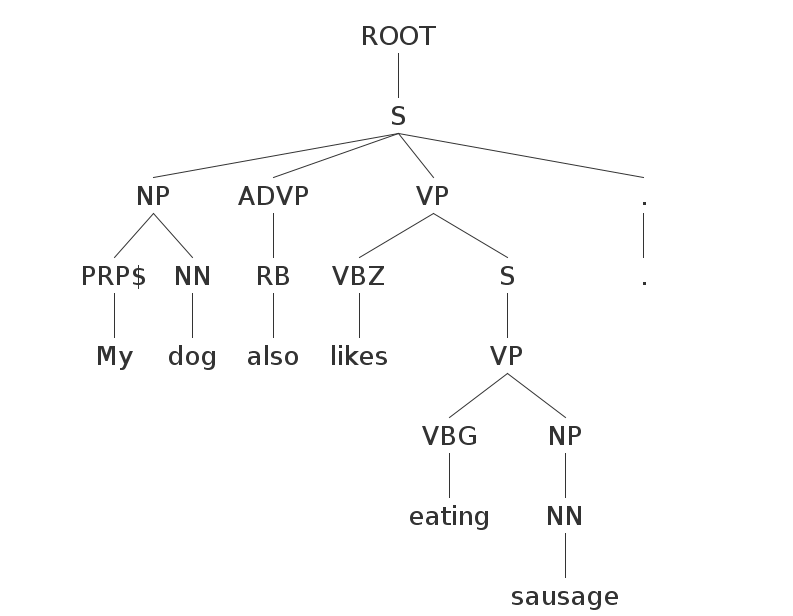
\includegraphics[scale=0.5]{tree}
 \subsection{Your own small Example}
 Running the same script, but with the sentence
 \begin{verbatim}
  The weather has been pretty bad lately.
 \end{verbatim}
 We will get the following text:
 \begin{verbatim}
  (ROOT
  (S
    (NP (DT The) (NN weather))
    (VP (VBZ has)
      (VP (VBN been)
        (ADJP (RB pretty) (JJ bad))
        (ADVP (RB lately))))
    (. .)))
 \end{verbatim}

 The graphical user interface yields the result: \\
 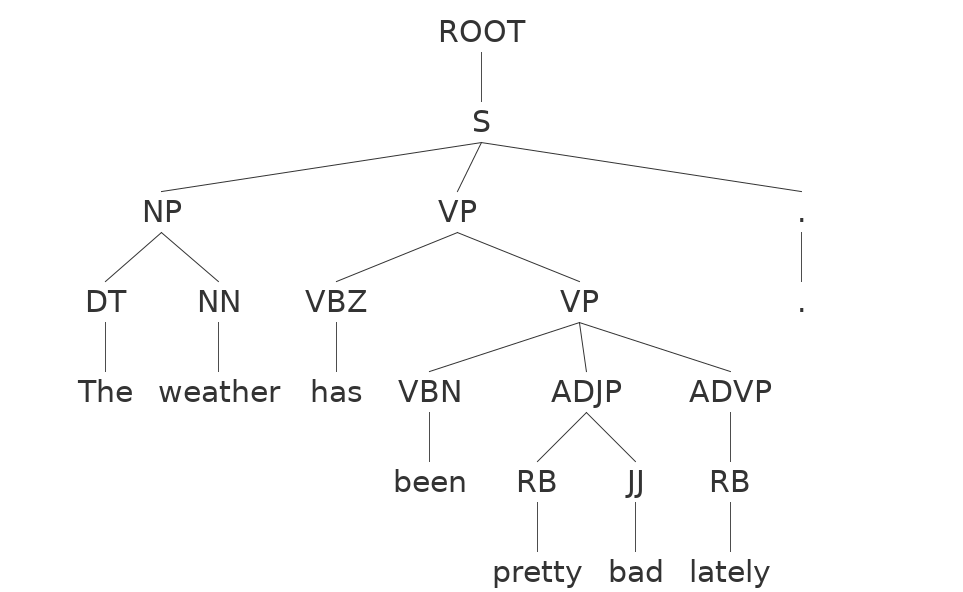
\includegraphics[scale=0.5]{tree2}
    
 
 \section{Proposed problem}
  \subsection{Specification} 
  The parser alone can't do much so, in order to solve a real problem, it must be used cojointly with the rest of the CoreNLP package. \\
  The proposed problem is the following: \\
  Given a piece of a news article, the tool will performs actions such as sentiment analysis, quote linking, coreference resolution, relation extraction, speaking time and named entity recognition. The result tree will also be displayed to the user and stored on a local hard drive, in order to have a visual representation of the in-memory data. \\
  A database will contain all the previously computed data. This will be useful for finding contradictions or other discrepancies. The tool should report all these discrepancies in order to ensure the correctness of the data. \\
  The aforementioned problems are discussed in the following articles: 
  
  \begin{itemize}
   \item \verb|https://edoc.hu-berlin.de/bitstream/handle/18452/2098/hamborg.pdf|
   \item \verb|http://www.scielo.br/pdf/interc/v39n1/en_1809-5844-interc-39-1-0039.pdf|
  \end{itemize}
  
  \subsection{Implementation} 
  The solution will be implemented as a Graphical Java application. It will consist of 2 parts: the MVC (Model, Controller, View) module for the GUI and the NLP (Natural Language Processing) for backend. \\
  The NLP module will be in charge of analysing incoming articles (documents comprising of multiple sentences) and will detect such things as referred dates and similarities to other articles. By detecting dates, we can detect whether the article is about a past, present or future event.
  The similarities can be detected by extracting the document's graph and computing it's cosine similarity / Euclidean distance to another article, giving an approximate view on whether two articles are related or not and, through model training, whether there is an entailment or contradiction. \\
  Data will be retrieved using the Webhose.io API, which is essentially a Java class which sends a request to a REST endpoint, and receives a JSON representation of a list of articles.

  \subsection{Documentation of your solution}
  Data received from the Webhost server is stored inside the program as instances of the Article class.
  This class contains information such as title, author, text, publish date, detected sentiment and times, quotes and a tree representation of the syntactic parser. \\
  When the user starts the application, he is presented with the graphical interface. He'll write a keyword in the text field and hit the `Search` button. After downloading the list of articles, the Stanford CoreNLP tool will analyse each article, and the user will be able to see the analysis results and also `star` certain articles. \\
  If the user chooses to star an article, each time the application is launched, each saved article is checked and, if it is detected that the article will be of interest to the user in the next 24 hours, a pop-up window with the specified articles will appear.


\end{document}          
